\documentclass[12pt,a4paper,twoside]{article}
\usepackage[utf8]{inputenc}
\usepackage[english]{babel}
\usepackage{amsmath}
\usepackage{amsfonts}
\usepackage{amssymb}
\usepackage{graphicx}
\usepackage[left=2cm,right=2cm,top=2cm,bottom=2cm]{geometry}

\usepackage{parcolumns}
\usepackage{siunitx}

\usepackage{pstricks}
\usepackage{pst-optexp}
\usepackage{xkeyval}

\author{Davide Bazzanella}
\title{Multidimensional Imaging of Ultrafast Laser Pulses}
%\institute{Imperial College London} 
\date{3$^{\mathrm{rd}}$ May 2016} 

\begin{document}
\pagenumbering{roman}	% numeration in roman numbers
\begin{titlepage}
\begin{center}

%\includegraphics[width=0.7\textwidth]{unitn_logo.png}~\\[1.2cm]

\hrule
$$$$
$$$$

\textsc{\LARGE \textbf{IMPERIAL COLLEGE LONDON}}\\[0.5cm]
\textsc{\LARGE \textbf{DEPARTMENT OF PHYSICS}}\\[1.3cm]
\textsc{\Large BSc PROJECT}\\[0.5cm]
\textsc{\Large Final Project Report}\\[1.3cm]

\vfill
\vfill
{ \huge \bfseries Multidimensional Imaging}\\
\vfill
{ \huge \bfseries of Ultrafast Laser Pulses}\\
\vfill
\vfill
\vfill

% WARNING! It need parcolumns package to work!
\begin{parcolumns}{2}
   \colchunk[1]{	
   				\Large Supervisor:\\
   				\LARGE \textbf{Tobias Witting}
   				}
   \colchunk[2]{
   				\Large Student:\\ \LARGE \textbf{Davide Bazzanella}
   				}
\end{parcolumns}
\vfill
\vfill
\vfill
\vfill
\vfill
\vfill
\vfill
\vfill
\vfill

\large ACADEMIC YEAR 2015/2016
\hrule
\vfill
\large TERM 2
\vfill
\vfill

\end{center}
\end{titlepage}
\cleardoublepage
\section*{Abstract}
%\begin{•}
We replicate a method for multidimensional characterisation of ultrafast laser pulses with slight variation.
The technique is based on Fourier transform spectral interferometry and is spatially resolved in three dimensions.

The sample beam is interfered with a copy of itself delayed and passed through a pinhole, therefore spatially uniform.
The interferogram is acquired on each pixel of a CMOS camera by scanning the delay between the sample and the reference pulse and allow us to gather high-resolution spatially resolved information on the phase difference between the two pulses.
This information is then elaborated by mean of Fourier transform along with the spectral amplitude and phase obtained with a SEA-F-SPIDER.

The result is a complete characterisation of the original pulse in three spatial dimensions (or two plus time).
\subsubsection*{Keywords:} Laser metrology, femtosecond pulses, ultrafast lasers, multidimensional characterisation, Fourier transform spectral interferometry
%\end{•}
\cleardoublepage
\tableofcontents

\cleardoublepage
\pagenumbering{arabic}
\section{Introduction}
%\begin{•}
Modern mode-locked lasers are able to generate ultrafast laser pulses with a duration down to few femtoseconds \cite{tamura93,schriever14,yu30} and with high repetition rates.
Those pulses are too short to be characterised by any present-day detector, therefore correlation, spectrographic and interferometric techniques are largely used in laser metrology.

Autocorrelation and cross-correlation are by far the most used methods, because of their simplicity.
These techniques are in fact the easiest techniques available, especially autocorrelation, but they allow to obtain only moderate information on the laser pulse.
Also they often need to assume the shape of test pulse to estimate its duration.

Among the spectrographic techniques, the most common one is the so called Frequency-Resolved Optical Gating (FROG).
This method involves measuring the spectrum of the test pulse as a function of the delay between its replicas.
Amplitude and phase information on the ultrashort pulse is then extracted using an interative-Fourier-transform algorithm.

Spectral-Phase Interferometry for Direct Electric-field Reconstruction (SPIDER) is an implementaton of shearing interferometry and is the most known interferometric method.
A SPIDER apparatus creates two replicas of the test pulse with a certain delay and mix them with the original pulse in a crystal with nonlinear properties (usually cut for Sum-Frequency Generation).
The output from the crystal is then analysed with a spectrometer and the complete reconstruction of the pulse is obtained through a direct algebraic relation with the data.
%tomography ?

These techniques are usually implemented considering the laser pulse transversely homogeneous.
This is often not the case, because distortions in the pulse spatial distribution may be introduced even by simple optical elements \cite{bor}.

Mutidimensional characterisation of a ultrafast laser pulse is often based on multiplexing of one of the forementione techniques.
To give an example, SPIDER can be easily multiplexed to characterise one spatial dimension and the time dependence of the ultrafast pulse.
FROG too can be scaled to allow also one spatial dimension characterisation.

Full (3D) characterisation of an ultrafast laser pulse require further multiplexing or mixing different techniques into a more complex one.
%\end{}

\subsection{Aims}
%\begin{•}
The aim of this project is to obtain a complete spatial and temporal characterisation of an ultrafast laser pulse, that is a three dimensional (3D) characterisation.
%The aim of this project is to spatially and temporally characterise an ultrafast laser pulse of \SI{3.5}{\fs} duration.

Our plan is to build a Mach-Zender interferometer to obtain a spatially resolved interferogram of the laser pulse, and convert it to the frequency domain via Fourier transform.
Then, by adding information on the frequency dependance of the phase and the amplitude, gathered using the SEA-F-SPIDER already available in the laboratory, we will characterise the beam spatial distribution in three dimensions.

The source to sample is a Ti:Sapphire laser which generates \SI{30}{\fs} pulses, successively spectrally broadened by a hollow core fiber and temporally compressed by broadband chirped mirrors into the final \SI{3.5}{\fs} pulse with a bandwidth that spans from \SI{500}{\nm} to \SI{1000}{\nm}.
%\end{}

\clearpage
\section{Fourier transform spectral interferometry}
Among the different techniques, we have chosen to develop a spatially resolved version of the Fourier transform spectral interferometry.
This method is based on the interference between the test beam and a reference beam, which is often a small homogeneous portion of a copy of the test pulse.

\subsection{Cross-correlation interferometry}
%\begin{•}
Consider an unknown laser pulse, its time complex field and the corresponding field in the spectral domain are given by
\begin{gather}
	U(t) = |U(t)|e^{i\phi(t)} \\
	\tilde{U}(\omega) = |\tilde{U}(\omega)|e^{i\psi(\omega)}
	\label{eq_def}
\end{gather}
which are linked together by Fourier transform $U(t) = \mathrm{FT}^{-1} \lbrace \tilde{U}(\omega) \rbrace$ and $\tilde{U}(\omega) = \mathrm{FT} \left\lbrace U(t) \right\rbrace$

Cross-correlation interferometry considers the pattern given by the intensity of the interference between two fields with a relative delay $\tau$.
The sensor measures the intensity of the fields over a time much longer than a single cycle, therefore we may write:
\begin{align}
	I(\tau) 	&= \int|U_1(t)+U_2(t-\tau)|^2\mathrm{d}t \nonumber\\
			&= \int|U_1(t)|^2\mathrm{d}t + \int|U_2(t)|^2\mathrm{d}t \nonumber\\
			&\quad + \int U_1(t)U_2^*(t-\tau)\mathrm{d}t + \int U_1^*(t)U_2(t-\tau)\mathrm{d}t 
	\label{eq_xcorr}
\end{align}
As we can see the first two terms are actually just the irradiance of the first beam $I_1 = \int|U_1(t)|^2\mathrm{d}t$ and of the second beam $I_2 = \int|U_2(t)|^2\mathrm{d}t$ and are therefore constant for each value of delay $\tau$.

Those component may be isolated and subtracted to the interferogram either by separate measurements or by removing the peak at $\omega = 0$ in the frequency domain.

The last two terms correlate the two fields together and afterwards may be adapted differently according to the approach chosen.
%\end{}

\subsection{Fourier transform spectral interferometry}
%\begin{•}
A special case of the cross-correlation interferometry is the test-plus-reference interferometry which tries to gather information on a test field $U(t)$ by correlating its interference pattern with a reference (known) field $U_r(t)$.
Our method, Fourier transform spectral interferometry, is the most common form of test-plus-reference interferometry.

Starting from cross-correlation intensity information and applying the Fourier transform to Eq. (\ref{eq_xcorr}) we obtain
%\begin{align}
%	\mathrm{FT} \lbrace I(\tau) \rbrace
%	&= \mathrm{FT} 	\left\lbrace	\int|U(t)|^2\mathrm{d}t + \int|U_r(t)|^2\mathrm{d}t +
%							\int U(t)U_r^*(t-\tau)\mathrm{d}t + \int U^*(t)U_r(t-\tau)\mathrm{d}t
%					\right\rbrace \nonumber\\
%	&= \mathrm{FT}	\left\lbrace \int|U(t)|^2\mathrm{d}t + \int|U_r(t)|^2\mathrm{d}t \right\rbrace
%	+ \tilde{U}(\omega)\tilde{U}_r^*(\omega)
%	+ \tilde{U}^*(-\omega)U_r(-\omega)
%	\label{eq_FTspectrum}
%\end{align}
\begin{align}
	\mathrm{FT} \lbrace I(\tau) \rbrace
	&= \mathrm{FT} 	\left\lbrace	
						\int|U(t)|^2\mathrm{d}t + \int|U_r(t)|^2\mathrm{d}t
					\right\rbrace \nonumber\\
	&+
		\mathrm{FT}	\left\lbrace	
						\int U(t)U_r^*(t-\tau)\mathrm{d}t
					\right\rbrace
	+	\mathrm{FT}	\left\lbrace	
						\int U^*(t)U_r(t-\tau)\mathrm{d}t
					\right\rbrace \\
	\label{eq_FTspectrum}
\end{align}
which, employing the convolution theorem, can be written as
\begin{align}
	\mathrm{FT} \lbrace I(\tau) \rbrace
	&= \mathrm{FT}	\left\lbrace \int|U(t)|^2\mathrm{d}t + \int|U_r(t)|^2\mathrm{d}t \right\rbrace \nonumber \\
	&+ \tilde{U}(\omega)\tilde{U}_r^*(\omega)
	+ \tilde{U}^*(-\omega)U_r(-\omega)
	\label{eq_FTspectrum1}
\end{align}
where $\tilde{U}(\omega)$ is the spectral domain complex field, as in Eq. (\ref{eq_def}).

The first term is the Fourier transform of a constant and is represented in the frequency domain by a peak at $\omega = 0$.
The second and third terms are represented by two peaks around $\omega_0$ and $-\omega_0$, where $\omega_0$ the main frequency of the pulse.
Figure (\ref{fig_spectrum}) is a representation from actual data in a lin-log scale of the spectrum amplitude.

\begin{figure}[h!]
	\centering
	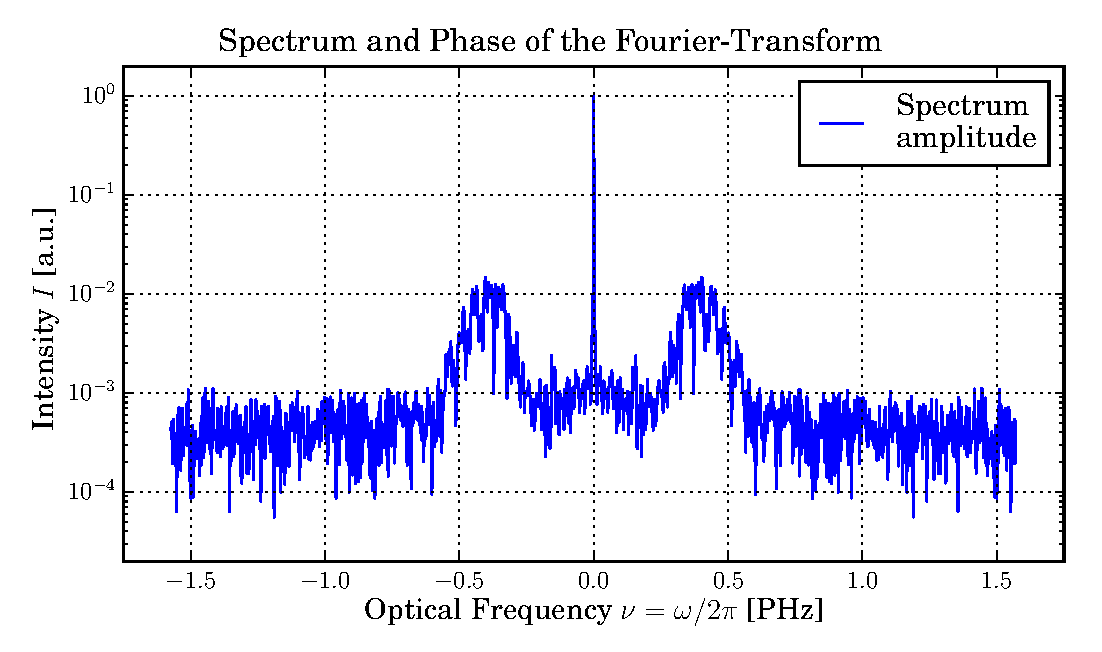
\includegraphics[scale=.9]{data/spectrum_linlog.eps}
	\caption{(Color Online) Spectrum amplitude of the interference pattern as a function of optical frequency $\nu$, in a lin-log scale to enhance the presence of the two terms in simmetrical position respect to the center.}
	\label{fig_spectrum}
\end{figure}

Considering only the second term, which can be isolated from the term at zero and its symmetric at $-\omega$, we can define:
\begin{align}
	A(\omega) 	&\equiv \mathrm{FT} \left\lbrace \int U(t)U_r^*(t-\tau)\mathrm{d}t \right\rbrace \\
				&= \tilde{U}(\omega)\tilde{U}_r^*(\omega) \nonumber\\
				&= |\tilde{U}(\omega)||\tilde{U}_r^*(\omega)|e^{i[\psi(\omega)-\psi_r(\omega)]}
\end{align}
%\begin{equation}
%	A(\omega) \equiv |\tilde{U}(\omega)||\tilde{U}_r^*(\omega)|e^{i[\psi(\omega)-\psi_r(\omega)]}
%\end{equation}
from which we can eventually get:
\begin{equation}
	\tilde{U}(\omega) = |\tilde{U}(\omega)|e^{i\psi(\omega)} = \frac{A(\omega)}{|\tilde{U}_r^*(\omega)|}e^{i\psi_r(\omega)}
\end{equation}

The steps described work for an ideal setup and for a one dimensional characterisation.
We will expand the theoretical description later in the subsection \textit{Multidimensional approach} of section \ref{sec_data_analysis}.
%\end{}

\section{System setup}
\subsection{Ultrafast laser pulses source}
%\begin{•}
Our source of ultrafast laser pulses is a Ti:Sapphire laser which generates pulses of \SI{30}{\fs} with an energy of \SI{700}{\milli\J} at a repetition rate of \SI{1}{\kHz}.
Those pulses are successively spectrally broadened in a \SI{1}{\m} long hollow fibre (\SI{250}{\um} inner core diameter) and then compressed in time by ultrabroadband chirped mirrors.
The compression is eventually fine-tuned by a pair of fused silica wedges, to obtain at the end of the process an ultrafast laser pulse of \SI{3.8}{\fs} duration and energy up to \SI{250}{\milli\J}.

The ultrafast laser pulse is generated on an optical table and then conveyed to our system, which is on a different optical table, through reflective optics only.

This source is rather unique and we had therefore to schedule its use compatibly with the other people in the research group.
%\end{}

\subsubsection*{HeNe CW laser}
%\begin{•}
We also used a continuous wave HeNe laser, generating a collimated red beam of wavelength $\lambda_{HeNe}=\SI{632.8}{\nm}$.
With its long coherence length and small beam waist was a useful prealignment tool.
%\end{}

\subsection{Mach-Zender interferometer}
%\begin{•}
\begin{figure}[ht]
	\centering
	\begin{pspicture}(14,10)
		\pnodes(0,8){IN}(14,4){OUT}
		\pnodes(2,8){BSA}(7,4){BSB}
		\pnodes(2,2){C}(4,2){D}(4,4){E}(6,4){Focus}
		\pnodes(11,8){G}(11,6){H}(7,6){I}
		
		\addtopsstyle{OptComp}{mirrorwidth=1.5, mirrortype=extended}
		\addtopsstyle{OptComp}{bssize=1.5, bsstyle=plate}
		\addtopsstyle{Beam}{fillstyle=solid, fillcolor=red!50!white, linecolor=red, opacity=0.2}
		
		\beamsplitter[labelangle=-135, labeloffset=1.5](IN)(BSA)(C){BS1}
		
		\mirror(BSA)(C)(D){M1}
		\mirror(C)(D)(E){M2}
		\oapmirror[oapmirroraperture=1.5, mirrortype=extended](D)(E)(Focus){OAP}
		\pinhole[outerheight=1,innerheight=0.1,phlinewidth=0.1](Focus)(Focus){PH}
		
		\beamsplitter[labelangle=45, labeloffset=1.5](I)(BSB)(OUT){BS2}
		
		\mirror(BSA)(G)(H){M3}
		\mirror(G)(H)(I){M4}
		\mirror(H)(I)(BSB){M5}
		
		\drawwidebeam[beamwidth=0.4](IN){1-6}(OUT)
		\drawwidebeam[beamwidth=0.4](IN)(BSA){7-9}{6}(OUT)
		
		\pnode(8,8){ND}
		\optbox[optboxsize=0.2 1.3, labeloffset=1](BSA)(ND){ND filter}		
		
		\optbox[optboxsize=4 4](8,7)(14,7)
		\rput[r](12.5,7.15){$\tau$\psline[arrows=<->](-0.65, -0.15)(0.35, -0.15)}
		\rput[c](11,9.5){moving platform}
		
		\rput[l](0,8){IN}
		\rput[r](14,4){OUT}
	\end{pspicture}
	\label{fig-MZ}
	\caption{(Color Online) Mach-Zender interferometer: BS1 and BS2 are the two 50/50 broadband beamsplitter, M1-5 are plain metallic mirrors, PH is the \SI{20}{\um} pinhole, OAP is the off-axis parabolic gold-plated mirror and ND is a neutral density filter (or a stack of filters).}
\end{figure}
\subsubsection*{Components}
\begin{itemize}
	\item 5$\times$ Ø1" metallic mirrors (M1, M2, M3, M4, M5)
	\item 1$\times$ Ø1" 90 off-axis parabolic mirror, protected gold coated (OAP)
	\item 2$\times$ Ø1" broadband 50/50 beamsplitter with antireflection coating
	\item 1$\times$ \SI{20}{\um} pinhole
	\item 1$\times$ moving platform with Zaber T-NA08 A 25 actuator
	\item 1$\times$ Allied Vision Guppy Pro F503B 12-bit 5MPixel CMOS camera
	\item 2$\times$ neutral density (ND) filters
	\item 1$\times$ 11$\times$16" steel breadboard
\end{itemize}
All the components have been fixed on the breadbord with common clamps, screws and washers.
All the mirrors have been mounted on pillars of the same height, exept for the two positioned on the the moving platform (M3, M4).
Those two mirrors, the beamsplitters and the pinhole have been mounted on pillars of different height to keep the center of the optical elements approssimately at the same height throughout the beam path.

\subsubsection*{Assembling}
%\begin{•}
The Mach-Zender interferometer was initially assembled with six plain mirrors and no pinhole.
To test the rough alignment of the two output beam, we used the HeNe gaussian beam because of its small waist and because it is relatively safer than the Ti:Sapphire.
Each arm had three mirrors to preserve the mirroring parity and to avoid retroreflection into the laser cavity.

Because we were working directly under a ventilation shaft we had to enclose the MZ in a box of black hardboard to avoid disturbances due to the air movement.

Due to the difficulties in alignment of the beam with the axis of movement of the platform, we decided to keep the reference arm fixed and build the moving platform in the test arm.
This choice avoided the problem of focusing the beam into the pinhole for every step of the platform.

After a preliminary stage we removed a plane mirror from one of the two arms and replaced with an off-axis parabolic mirror and a pinhole.

%\end{}

\subsection{SEA-F-SPIDER}
%\begin{•}
In the laboratory a variation from the traditional SPIDER apparatus was already available: spatially encoded arrangement for direct electric field reconstruction by spectral shearing interferometry (SEA-SPIDER) with direct spatial filtering for ancilla preparation (SEA-F-SPIDER).

This apparatus, compared to SPIDER, is particularly fitted for few-cycle pulse characterisation and is able to reconstruct the time dependence and the spatial distribution in one dimension of the pulse.
%\end{}

\clearpage
\section{Data Analysis}
\label{sec_data_analysis}
%\begin{•}
Our output data is composed by the interferograms of each pixel of the camera and from the amplitude and phase frequency dependence gathered by the SEA-F-SPIDER.
All the interferograms are arranged in a big 3D matrix, whose dimension are given by the resolution of the sensor and the number of steps from the samplig in the delay line.
Considering a 12-bit color (greyscale) depth and the original resolution of the camera ($2588\times 1940$), the memory usage of the raw data for 1024 sampling steps is more than 7 GB.
To keep memory usage lower we binned together pixels in $4\times 4$ groups obtaining an effective resolution of $647\times 485$ and a reduction of a factor 16 in the memory usage.
During the code developing and debugging phases we reduced the memory usage further by cropping the resolution to $201\times 201$ in the center of the sensor.
%\end{}

\subsection{Multidimensional approach}
%\begin{•}
\begin{equation}
	\tilde{U}(x,y,\omega) = \frac{A(x,y,\omega)}{|\tilde{U}_r^*(x,y,\omega)|}e^{i\psi_r(x,y,\omega)}
\end{equation}
assumptions:
\begin{itemize}
\item the intensity of the reference beam is homogeneous in the transverse directions $|\tilde{U}(x,y,\omega)|=|\tilde{U}(x_0,y_0,\omega)|=|\tilde{U}(\omega)|$ where ($x_0$,$y_0$) are the coordinates of the center of the beam.
\item the phase is separable as a spatial component and an angular frequency component:\\ $\psi_r(x,y,\omega) = \psi_{r,sp}(x,y)\psi_{r,\omega}(\omega)$
\end{itemize}
Then:
\begin{equation}
	\tilde{U}(x,y,\omega) \approx \frac{A(x,y,\omega)}{|\tilde{U}_r^*(\omega)|}e^{i\psi_r(x,y)}e^{i\psi_r(\omega)}
\end{equation}

The first assumption is valid because the reference beam is created by focusing the beam into a \SI{20}{\um} pinhole.
This produces on the camera sensor an Airy pattern.
As a first approximation the central area of the pattern may be considered homogeneous in intensity.
This area is the Airy disk which has a radius given by
$$\rho_s = 1.22 \frac{\lambda d}{D}$$
where $\lambda$ is the wavelength, $d$ is the distance between the aperture and camera and $D$ is the diameter of the aperture.\\
In our experiment the worst case values are $\lambda = \SI{500}{\nm}$, $D = \SI{20}{\um}$ and $d \approx \SI{300}{\mm}$ and give $\rho_s = \SI{9.15}{\mm}$ which is greater than both the height and the width of the sensor ($4 \times 6 \si{\mm}$)

The second assumption helds if air is considered a non dispersive medium, which is true throughout this discussion
%\end{}

\subsection{Code development}
%\begin{}
\subsubsection*{Acquisition code}
we controlled the apparatus through MATLAB script
after the first data acquisitions we discovered that the attuator corrupted the first points of the data due to its backlash at the initial position.
We solved the problem by moving the attuator further back and forcing him to take a few steps in the right direction before placing it on the first sampling position.

\subsubsection*{Processing code}
data was processed with a second MATLAB script
%\end{}

\clearpage
\section{Conclusions}
\subsection{Improvements}
%\begin{•}
As a technical improvement corner cube rectroreflector may be used for a better alignment and less sensibility to the mirrors movement.

The use of corner cube retroreflectors, depending on the kind employed, may lead to parity problems, as the beam may not reflect the same number of times in both arms.
In our system, though, this is not a problem, as the presence of the pinhole eliminate any symmetry problem.

To eliminate the needs of a numerical phase correction there are two possible ways.
A solution is to remove the filter and substitute the first beamsplitter with one which conveys more energy to the reference arm than to the test arm.
To obtain a disrete fringe contrast, though, the energy in the two arms should be as similar as possible.
Given the fact that we obtained good fringes contrast with a stack of heavy (ND up to optical density $d=5$), it means that we need a beamsplitter which transmit $10^{-5}$ of the incident intensity and reflects the remaining ($\simeq 1$).
Another solution is to balance the two arms by adding a slab of the same material and thickness of the ND filter in the test arm.

Both solutions lead to the generation of a interferogram with thinner fringes.
This is a problem because the attuator we used in the esperiment has a minimum step of \SI{47.625}{\nm}, which is not enough small for the resolution required by the new interferogram.

*** formula per calcolare il minimo step richiesto ***
%\end{}

\subsection{Personal considerations}
%\begin{}
Much time was spent in aligning the output beams, moving mirrors

due to the precision required by such extreme condition (\si{\fs}, \si{\nm})

At the beginning, I had to become familiar with the environment and the equipement in the
laboratory.

working in an actual research environment

even though we did not obtain the results we did hope to

formative experience
%\end{}

\clearpage
\begin{thebibliography}{99}
\bibitem{tamura93} Tamura, K., et al. "77-fs pulse generation from a stretched-pulse mode-locked all-fiber ring laser." Optics letters 18.13 (1993): 1080-1082.
\bibitem{schriever14} Schriever, Christian, et al. "Tunable pulses from below 300 to 970 nm with durations down to 14 fs based on a 2 MHz ytterbium-doped fiber system." Optics letters 33.2 (2008): 192-194.
\bibitem{yu30} Yu, Tae Jun, et al. "Generation of high-contrast, 30 fs, 1.5 PW laser pulses from chirped-pulse amplification Ti: sapphire laser." Optics express 20.10 (2012): 10807-10815.
\bibitem{bor} Bor, Zsolt. "Distortion of femtosecond laser pulses in lenses." Optics letters 14.2 (1989): 119-121.
\bibitem{miranda} Miranda, Miguel, et al. "Spatiotemporal characterization of ultrashort laser pulses using spatially resolved Fourier transform spectrometry." Optics letters 39.17 (2014): 5142-5145.
\bibitem{walmsley} Walmsley, Ian A., and Christophe Dorrer. "Characterization of ultrashort electromagnetic pulses." Advances in Optics and Photonics 1.2 (2009): 308-437.
\bibitem{witting} Witting, Tobias, et al. "Characterization of high-intensity sub-4-fs laser pulses using spatially encoded spectral shearing interferometry." Optics letters 36.9 (2011): 1680-1682.
\bibitem{trebino} Trebino, Rick, and Daniel J. Kane. "Using phase retrieval to measure the intensity and phase of ultrashort pulses: frequency-resolved optical gating." JOSA A 10.5 (1993): 1101-1111.


\end{thebibliography}
\end{document}
